\documentclass{article}
\usepackage[landscape,letterpaper,left=1cm,right=1cm,top=1cm,bottom=1cm]{geometry}

\usepackage{booktabs}
\usepackage{color}
\usepackage[type={CC},modifier={by-sa},version={4.0}]{doclicense}
\usepackage[inline,shortlabels]{enumitem}
\usepackage{graphicx}
\usepackage{multicol}
\usepackage{parskip}            % stop indenting
\usepackage{url}

\usepackage[compact]{titlesec}
\titleformat{\section}{\normalfont\fontsize{12}{15}\bfseries}{\thesection}{0ex}{}
\titlespacing{\section}{0pt}{0.5ex}{0.5ex}
\titleformat{\subsection}{\normalfont\fontsize{9}{12}\bfseries}{\thesection}{0ex}{}
\titlespacing{\subsection}{0pt}{0.5ex}{0.5ex}

\usepackage{fancyhdr}
\pagestyle{empty}

\usepackage{xltxtra}
\setmainfont[Ligatures=TeX]{Helvetica Neue}
\setmonofont[AutoFakeSlant,BoldItalicFeatures={FakeSlant}]{Courier}

\usepackage{listings}
\lstdefinelanguage{plain}{%
  basicstyle=\ttfamily,
  keywordstyle={},
  identifierstyle={},
  commentstyle={},
  stringstyle={},
  numbers=left,
  frame=single}
\lstset{
  belowskip=0.2em,
  aboveskip=0.2em,
  language=plain,
  basicstyle=\ttfamily
}

\begin{document}

\raggedright

\begin{multicols*}{3}
  \footnotesize

  \begin{center}
    {\Large{}\bfseries{}Go Reference Card}

    Dr. Nicholas M. Boers\\
    \url{boersn@macewan.ca}\\
    \IfFileExists{macewan.pdf}{
      \vspace{0.2em}
      
\includegraphics[height=0.85cm]{macewan}
    }{
      MacEwan University
    }

    \vspace{1em}
    Last updated: \today
  \end{center}

  \filbreak
  \section*{Introduction}

  \subsection*{Synopsis}

  \texttt{go command [arguments]}

  \subsection*{Commands (basic)}

  \begin{tabular}{p{0.5in}p{2.5in}}
    \toprule
    \textbf{Command} & \textbf{Description} \\
    \midrule
    \texttt{build} & compile packages and dependencies \\
    \texttt{get} & download and install packages and dependencies \\
    \texttt{run} & compile and run Go program \\
    \bottomrule
  \end{tabular}

  \subsection*{Program execution}

  Execution begins at the function \texttt{main} in package \texttt{main}:
\begin{lstlisting}[numbers=none,escapechar=\%]
package main

func main() {
    % \dots%
}
\end{lstlisting}

  \filbreak
  \section*{Variables}

  \subsection*{Types (basic)}

  \begin{tabular}{p{0.5in}p{2.5in}}
    \toprule
    \textbf{Type} & \textbf{Description} \\
    \midrule
    \texttt{string} & sequence of bytes (immutable)\newline{}
                      \texttt{"\dots"}: interpreted string literal\newline{}
                      \texttt{`\dots`}: raw string literal (no backslash escapes)\\
    \texttt{bool} & Boolean value; either \texttt{true} or \texttt{false} \\
    \texttt{int\textit{\underbar{x}}} & signed \texttt{\textit{\underbar{x}}}-bit integer where \texttt{\textit{\underbar{x}}} is 8, 16, 32, or 64 \\
    \texttt{uint\textit{\underbar{x}}} & unsigned \texttt{\textit{\underbar{x}}}-bit integer \\
    \texttt{float\textit{\underbar{x}}} & \texttt{\textit{\underbar{x}}}-bit float where \texttt{\textit{\underbar{x}}} is 32 or 64 \\
    \bottomrule
  \end{tabular}

  \subsection*{Declarations}

  \begin{tabular}{p{0.75in}p{2.25in}}
    \toprule
    \textbf{Syntax} & \textbf{Description} \\
    \midrule
    \texttt{var \textit{\underbar{id}} \textit{\underbar{type}}} & declare identifier \texttt{\underbar{id}} as \texttt{\underbar{type}} \\
    \bottomrule
  \end{tabular}

  \filbreak
  \section*{Keywords}

  \begin{tabular}{p{0.5in}p{0.65in}p{0.35in}p{0.5in}p{0.5in}}
    \texttt{break}    & \texttt{default}     & \texttt{func}   & \texttt{interface} & \texttt{select} \\
    \texttt{case}     & \texttt{defer}       & \texttt{go}     & \texttt{map}       & \texttt{struct} \\
    \texttt{chan}     & \texttt{else}        & \texttt{goto}   & \texttt{package}   & \texttt{switch} \\
    \texttt{const}    & \texttt{fallthrough} & \texttt{if}     & \texttt{range}     & \texttt{type} \\
    \texttt{continue} & \texttt{for}         & \texttt{import} & \texttt{return}    & \texttt{var} \\
  \end{tabular}

  \filbreak
  \section*{Operators, delimiters, and other tokens }

  Operators, delimiters, and other special tokens available:

  \begin{tabular}{lllllllll}
    \verb!+! & \verb!& ! & \verb!+=! & \verb!&= ! & \verb!&&! & \verb+==+ & \verb+!= + & \verb!(! & \verb!)! \\
    \verb!-! & \verb!| ! & \verb!-=! & \verb!|= ! & \verb!||! & \verb+< + & \verb+<= + & \verb![! & \verb!]! \\
    \verb!*! & \verb!^ ! & \verb!*=! & \verb!^= ! & \verb!<-! & \verb+> + & \verb+>= + & \verb!{! & \verb!}! \\
    \verb!/! & \verb!<<! & \verb!/=! & \verb!<<=! & \verb!++! & \verb+= + & \verb+:= + & \verb!,! & \verb!;! \\
    \verb!%! & \verb!>>! & \verb!%=! & \verb!>>=! & \verb!--! & \verb+! + & \verb+...+ & \verb!.! & \verb!:! \\
    \verb! ! & \verb!&^! & \verb!  ! & \verb!&^=! & \verb!  ! & \verb+  + & \verb+   + & \verb! ! & \verb! ! \\
  \end{tabular}

  Notable differences from C:

  \begin{tabular}{ll}
    \texttt{\&\textasciicircum} & bit clear (AND NOT) \\
    \texttt{\&\textasciicircum=} & bit clear (AND NOT) to update a variable \\
    \texttt{<-} & channel send/receive \\
    \texttt{:=} & short variable declaration     \\
  \end{tabular}

  \filbreak
  \section*{Functions}

  \subsection*{Syntax (basic)}

  \begin{lstlisting}[numbers=none,escapechar=\%]
func %\textit{\underbar{name}}%(%\textit{\underbar{arguments}}%) %\textit{\underbar{return type}}% {
    %\dots%
}
\end{lstlisting}

  \filbreak
  \section*{Control structures}

  \subsection*{\texttt{if} statement}

  \lstinline{if} statements provide conditional execution.

  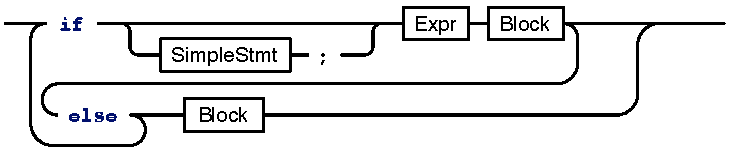
\includegraphics[width=\linewidth]{if}

  \begin{description}
  \item[Expr] expression, similar to C (e.g.,~\lstinline{1 + 2 * 3})
  \item[SimpleStmt] expression, increment/decrement statement (e.g.,~\lstinline{i++}), assignment (e.g.,~\lstinline{count = 0}), short declaration (e.g.,~\lstinline{count := 0})
  \item[Block] statement list inside braces, similar to C (e.g.,~\lstinline!{ count := 0; }!)
  \end{description}

  \filbreak
  \subsection*{\texttt{for} statement}

  \lstinline{for} statements provide repetition.
  The first form is similar to C with its three part: initialization, condition, and update.
  The second form is similar to C's \texttt{while} loop.
  The third form shares similarities with Python's \lstinline{for} loop.

  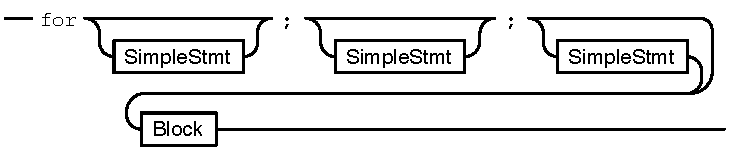
\includegraphics[width=\linewidth]{for-3parts}

  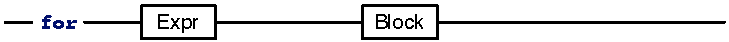
\includegraphics[width=\linewidth]{for-1cond}

  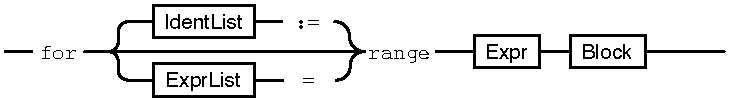
\includegraphics[width=\linewidth]{for-range}

  \begin{description}
  \item[IdentList] identifiers separated by commas (e.g.,~\lstinline{i, j, k})
  \item[ExprList] expressions separated by commas (e.g.,~\lstinline{key, val})
  \end{description}

  \filbreak
  \subsection*{\lstinline{switch} statement}

  \lstinline{switch} statements provide conditional execution.

  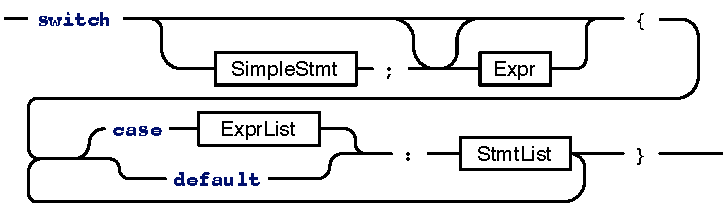
\includegraphics[width=\linewidth]{switch-expr}

  \filbreak
  \section*{Standard library}

  \begin{tabular}{p{0.8in}p{2.2in}}
    \toprule
    \textbf{Package} & \textbf{Description} \\
    \midrule
    \texttt{database/sql} & generic interface around SQL DBs \\
    \texttt{encoding/csv} & read/write CSV files \\
    \texttt{encoding/json} & encode/decode JSON \\
    \texttt{errors} & manipulation of errors \\
    \texttt{flag} & command-line argument parsing \\
    \textbf{\texttt{fmt}} & formatted I/O, e.g., \texttt{Printf} \\
    \texttt{log} & simple logging\\
    \texttt{math/rand} & pseudo-random number generators \\
    \textbf{\texttt{net/http}} & HTTP client/server implementations \\
    \texttt{os} & interface to OS functionality \\
    \texttt{path} & manipulation of slash-separated paths \\
    \texttt{sort} & primitives for sorting \\
    \textbf{\texttt{strings}} & string manipulation (UTF-8 encoded) \\
    \texttt{time} & functionality for measuring/displaying time \\
    \bottomrule
  \end{tabular}

  \filbreak
  \section*{Pointers}

  \filbreak
  \section*{map}

  \filbreak
  \section*{slices}

  \filbreak
  \section*{struct}

  \filbreak
  \section*{User-defined types}

  \filbreak
  \section*{Methods}

  \filbreak
  \section*{Interfaces}

  \filbreak
  \section*{Error}

  \parbox{\columnwidth}{
    Sources:
    \begin{itemize}[nosep]
    \item \texttt{go --help}
    \item \url{https://golang.org/ref/spec}
    \end{itemize}

    \vspace{\baselineskip}
    \begin{center}
      \doclicenseText\\[0.25\baselineskip]

      \doclicenseImage
    \end{center}
  }
\end{multicols*}

\end{document}
